%\documentclass[12pt,t]{beamer}
% \documentclass[t]{beamer}
\documentclass[handout]{beamer}\usepackage[]{graphicx}\usepackage[]{color}
%% maxwidth is the original width if it is less than linewidth
%% otherwise use linewidth (to make sure the graphics do not exceed the margin)
\makeatletter
\def\maxwidth{ %
  \ifdim\Gin@nat@width>\linewidth
    \linewidth
  \else
    \Gin@nat@width
  \fi
}
\makeatother

\definecolor{fgcolor}{rgb}{0.345, 0.345, 0.345}
\newcommand{\hlnum}[1]{\textcolor[rgb]{0.686,0.059,0.569}{#1}}%
\newcommand{\hlstr}[1]{\textcolor[rgb]{0.192,0.494,0.8}{#1}}%
\newcommand{\hlcom}[1]{\textcolor[rgb]{0.678,0.584,0.686}{\textit{#1}}}%
\newcommand{\hlopt}[1]{\textcolor[rgb]{0,0,0}{#1}}%
\newcommand{\hlstd}[1]{\textcolor[rgb]{0.345,0.345,0.345}{#1}}%
\newcommand{\hlkwa}[1]{\textcolor[rgb]{0.161,0.373,0.58}{\textbf{#1}}}%
\newcommand{\hlkwb}[1]{\textcolor[rgb]{0.69,0.353,0.396}{#1}}%
\newcommand{\hlkwc}[1]{\textcolor[rgb]{0.333,0.667,0.333}{#1}}%
\newcommand{\hlkwd}[1]{\textcolor[rgb]{0.737,0.353,0.396}{\textbf{#1}}}%
\let\hlipl\hlkwb

\usepackage{framed}
\makeatletter
\newenvironment{kframe}{%
 \def\at@end@of@kframe{}%
 \ifinner\ifhmode%
  \def\at@end@of@kframe{\end{minipage}}%
  \begin{minipage}{\columnwidth}%
 \fi\fi%
 \def\FrameCommand##1{\hskip\@totalleftmargin \hskip-\fboxsep
 \colorbox{shadecolor}{##1}\hskip-\fboxsep
     % There is no \\@totalrightmargin, so:
     \hskip-\linewidth \hskip-\@totalleftmargin \hskip\columnwidth}%
 \MakeFramed {\advance\hsize-\width
   \@totalleftmargin\z@ \linewidth\hsize
   \@setminipage}}%
 {\par\unskip\endMakeFramed%
 \at@end@of@kframe}
\makeatother

\definecolor{shadecolor}{rgb}{.97, .97, .97}
\definecolor{messagecolor}{rgb}{0, 0, 0}
\definecolor{warningcolor}{rgb}{1, 0, 1}
\definecolor{errorcolor}{rgb}{1, 0, 0}
\newenvironment{knitrout}{}{} % an empty environment to be redefined in TeX

\usepackage{alltt}
\usepackage{pgfpages}
\usepackage{pgffor}
\pgfpagesuselayout{4 on 1}[a4paper,landscape]

\pagestyle{empty} % descomentar para impresión muy blanca

\usepackage[utf8]{inputenc}
\usepackage[spanish]{babel}
\decimalpoint
\usepackage{verbatim}
\usepackage{hyperref}
%\hypersetup{colorlinks=false,linkbordercolor=red,linkcolor=green,pdfborderstyle={/S/U/W 1}}
%\hypersetup{colorlinks=true,linkbordercolor=red,linkcolor=green,pdfborderstyle={/S/U/W 1}}
\hypersetup{colorlinks=true,linkcolor=blue,pdfborderstyle={/S/U/W 1}}

\usepackage{amsfonts,amssymb,amsmath,amsthm, wasysym}
\usepackage{listings}
%\usepackage[T1]{fontenc}        
\usepackage{pgf}
%\usepackage{epsdice}
\usepackage{pgfpages}
\usepackage{tikz}
\usetikzlibrary{arrows,shapes,plotmarks,backgrounds,trees,positioning}
\usetikzlibrary{decorations.pathmorphing,calc,snakes}
%\usepackage{marvosym}
%
\usetheme[hideothersubsections,left]{Marburg}
%\usetheme[hideothersubsections,left]{Madrid}
%\usetheme[hideothersubsections,left]{Dresden}
%\usetheme{Darmstadt}
\usecolortheme{sidebartab}
\useinnertheme[shadow]{rounded}

% \useoutertheme[footline=empty,subsection=true,compress]{infolines}
% \useoutertheme[footline=empty,subsection=true,compress]{miniframes}
% \usefonttheme{serif}

\setbeamertemplate{caption}[numbered]
%\setbeamertemplate{navigation symbols}{}
\addtobeamertemplate{navigation symbols}{}{%
    \usebeamerfont{footline}%
    \usebeamercolor[fg]{footline}%
    \hspace{1em}%
    \insertframenumber/\inserttotalframenumber
    
    \setbeamercolor{footline}{fg=blue}
\setbeamerfont{footline}{series=\bfseries}
}

\newcommand{\red}[1]{\textcolor{red}{#1}}
\newcommand{\green}[1]{\textcolor{green}{#1}}
\newcommand{\blue}[1]{\textcolor{blue}{#1}}
\newcommand{\gray}[1]{\textcolor{gray}{#1}}
\renewcommand{\emph}[1]{{\color{red}#1}}

%\newtheorem{theorem}



\setbeamertemplate{frametitle}
{\begin{centering}
\medskip
\color{blue}
\textbf{\insertframetitle}
\medskip
\end{centering}
}
\usecolortheme{rose}
\usecolortheme{dolphin}
\mode<presentation>


\newcommand{\CC}{\mathbb{C}}
\newcommand{\RR}{\mathbb{R}}
\newcommand{\ZZ}{\mathbb{Z}}
\newcommand{\NN}{\mathbb{N}}
\newcommand{\KK}{\mathbb{K}}
\newcommand{\MM}{\mathcal{M}}
%\newcommand{\dbinom}{\displaystyle\binom}

\newcommand{\limn}{{\displaystyle lim_{n\to\infty}}}

%\renewcommand{\lim}{\displaystyle \mathrm{lim}}
\renewcommand{\leq}{\leqslant}
\renewcommand{\geq}{\geqslant}
\def\tendeix{{\displaystyle\mathop{\longrightarrow}_{\scriptscriptstyle
n\to\infty}}}

\newcommand{\matriu}[1]{\left(\begin{matrix} #1 \end{matrix}\right)}

% \newcommand{\qed}{\hbox{}\nobreak\hfill\vrule width 1.4mm height 1.4mm depth 0mm
%     \par \goodbreak \smallskip}
%
% %

\theoremstyle{plain}
\newtheorem{teorema}{Teorema}
%\newtheorem{prop}{Proposición}
\newtheorem{prop}{Propiedades}
\newtheorem{cor}{Corolario}
\theoremstyle{definition}
\newtheorem{ejemplo}{Ejemplo}
\newtheorem{definicion}{Definición}
\newtheorem{obs}{Observación}

\newcounter{seccions}
\newcommand{\seccio}[1]{\addtocounter{seccions}{1}
\medskip\par\noindent\textbf{\theseccions.
#1}\smallskip\par }

\newcommand{\EM}{\Omega}
\newcommand{\PP}{\mathcal{P}}

\title[\red{Matemáticas III GINF}]{}
\author[]{R. Alberich}
\date{}
\IfFileExists{upquote.sty}{\usepackage{upquote}}{}
\begin{document}
\beamertemplatedotitem

\lstset{backgroundcolor=\color{green!50}}
\lstset{breaklines=true}
\lstset{basicstyle=\ttfamily}


\section{Variables Aleatorias}

\begin{frame}
\vfill
\begin{center}
\gray{\LARGE Distribuciones notables II }
\end{center}
\vfill
\end{frame}

\subsection{Distribución Poisson}

\begin{frame}
\frametitle{Distribución Poisson}
\begin{itemize}
\item  Diremos que una v.a. discreta $X_t$ con $X(\Omega)=\NN$ tiene
distribución de Poisson con parámetro $\lambda>0$, y lo denotaremos
por $Po(\lambda)$ si su función de probabilidad es:

$$P_{X_t}(x)=P(X_t=x)=
\left\{\begin{array}{ll}
\frac{\lambda^x}{x!} e^{-\lambda}& \mbox{ si } x=0,1,\ldots\\
0 & \mbox{en otro caso}\end{array}\right..$$

\item Como el desarrollo en serie  Taylor de la exponencial es 
$$e^{\lambda}=\sum_{x=0}^{+\infty} \frac{\lambda^x}{x!}.$$
\item Es fácil comprobar que  todos los valores de la función de probabilidad suman 1 (ejercicio).
\end{itemize}
\end{frame}


\subsubsection{La distribución Poisson como ``límite'' de una binomial.}

\begin{frame}

\frametitle{La distribución Poisson como ``límite'' de una binomial.}

\begin{itemize}
\item La distribución Poisson aparece en el conteo de determinados  eventos que se
producen en un intervalo de tiempo o en el espacio.
\item Supongamos que nuestra variable de interés es  
$$X= \mbox{número de eventos en el intervalo de tiempo} (0,t].$$ 
\item Por ejemplo el número de
llamadas a un \textsl{call center} del que sabemos que se
cumplen las  condiciones siguientes:
\end{itemize}
\end{frame}



\begin{frame}
\frametitle{Condiciones para la distribución Poisson.}
\begin{enumerate}[a)]
\item El número promedio de eventos en el intervalo $(0,t]$ es
$\lambda>0$.
\item Es posible dividir el intervalo de tiempo en un
gran número de subintervalos (denotemos por $n$ al número de intervalos) de forma que:
\begin{enumerate}[1)]
\item La probabilidad de que se produzcan dos o más eventos en un
subintervalo es despreciable.
\item El número de ocurrencias de eventos en un intervalo  es
independiente del número de ocurrencias en otro intervalo.
\item La probabilidad de que un evento ocurra en un subintervalo
es $p=\frac{\lambda}{n}$·
\end{enumerate}
\end{enumerate}
\end{frame}

\begin{frame}

\frametitle{La distribución Poisson como límite de una distribución binomial (\emph{OPCIONAL})}
\begin{itemize}
\item Bajo estas condiciones podemos considerar que el número de eventos en
el intervalo $(0,t]$ será el número de ``éxitos'' en $n$
repeticiones independientes de un proceso Bernoulli de parámetro
$p$
\item  Entonces si $n\to\infty$ y $p\cdot n$ se mantiene igual a $\lambda$
resulta que la función de probabilidad de $X$ se puede poner como

$$f_{X}(k)=\lim_{n\to\infty}\left(\begin{array}{c} n\\ k\end{array}\right)
p^k q^{n-k}= \frac{\lambda^k}{k!} e^{-\lambda}$$
\end{itemize}
\end{frame}


\begin{frame}
\frametitle{Aproximación de la distribución binomial por la Poisson:}
Bajo el punto de vista anterior y si $p$ es pequeño y $n$
suficientemente grande (existen distintos criterios por ejemplo $n>20$ ó $30$ y  $p\geq 0.1$, $1-p\geq 0.1$)
podemos aproximar una $B(n,p)$ por una $Po(n\cdot p)$
\end{frame}

\begin{frame}
\frametitle{Los procesos Poisson.}
\begin{prop}
Si tenemos un experimento \emph{Poisson}  con $\lambda$ igual
al promedio de eventos en una unidad de tiempo (u.t.) entonces si

$$ t \mbox{ es una cantidad de tiempo en u.t., la v.a}$$
$$X_{t}=\mbox{numero de eventos en el intervalo} (0,t] 
\mbox{es una } Po(\lambda\cdot t).$$
\end{prop}

  A la familia de variables $X_t$ se la denomina proceso de Poisson.
\end{frame}

\begin{frame}
\frametitle{Resumen v.a con distribución  Poisson  $Po(\lambda)$}
\scriptsize
\setlength{\tabcolsep}{1pt}
\begin{table}
\centering
\begin{tabular}{|rl|}
\hline 
\multicolumn{2}{|c|}{$X$ Poisson $\lambda$.}\\ 
\hline
\hline 
$D_X=$&  $\{0,1,\ldots n\}$ \\\hline 
$P_X(x)=P(X=x)=$ & 
$\left\{
\begin{array}{ll}
  \frac{\lambda^x}{x!}\exp{-\lambda} & \mbox{ si } x=0,1,\ldots,n\\
     0  & \mbox{ en otro caso.}
     \end{array}\right.$
\\ \hline 
$F_X(x)=P(X\leq X)=$ &  Función de R o tabulada \\\hline 
$E(X)=$ &  $\lambda$ \\
$Var(X)=$ & $\lambda$\\
\hline
\end{tabular}
\end{table}
\normalsize
\end{frame}


\begin{frame}
\frametitle{Ejemplos procesos de Poisson}
Podrían, aunque no siempre, seguir una distribución Poisson las siguientes situaciones
\begin{itemize}
\item Número de conexiones a un \textsl{web service}.
\item Numero de erratas  por página en un libro.
\item Número de clientes en la cola de un cajero de un supermercado.
\item Número de insectos capturados en una trampa en un cierto intervalo de tiempo.
\item Número de errores en la clasificación de miles de fotografías de una red neuronal....
\end{itemize}
\end{frame}

\begin{frame}
\frametitle{Ejercicio}

\emph{$P(X=x)=\frac{\lambda^x}{x!}\cdot e^{-\lambda}$}

Supongamos que disponemos de un servicio de correo electrónico y que estamos interesados en contar el número de correos no deseado (SPAM) que recibimos. Supongamos que recibimos 2 correos no deseados por  minuto.

¿Cuál es la probabilidad de que en 4 minutos recibamos exactamente 3 correos no deseados?


$X_t$=número de correos no deseados en $t$ minutos.


Supongamos que es un proceso de Poisson $X_t$ con parámetro 
$\lambda_t=\lambda\cdot t=2\cdot  t.$

$X_4=$ número de correos no deseados en 4 minutos es una $Po(2\cdot 4)$.

$P(X_4=3)=\frac{8^3}{3!}\cdot e^{-8}=0.0286$.
\end{frame}

\begin{frame}
\frametitle{Ejercicio: Alquiler  vacacional}

La empresa \textsl{Alquilo Beds} (AB)   es un servicio de alquiler de apartamentos vacacionales por Internet.

El número de alquileres  en  el pueblo de la Colonia de Sant Antoni  por día a través de AB es de  $1.5$.

\begin{itemize}
\item ¿Cuál es la probabilidad de que en una semana  no se alquile ningún apartamento a través de AB?
\item ¿Cuál es la probabilidad de que en 15 días se alquilen como mínimo 2 apartamentos mediante  AB?
\end{itemize}
\end{frame}

\begin{frame}
\frametitle{Ejercicio: Alquiler  vacacional}

La empresa \textsl{Alquilo Beds} (AB)   es un servico de alquiler de apartamentos vacacionales por internet.

El número de alquileres  en  el pueblo de la Colonia de Sant Antoni  por día a través de AB es de  $1.5$.

$X_t=$ número de apartamentos alquilados en $t$ días, supongamos que es $Po(1.5\cdot t)$.


\begin{itemize}
\item ¿Cuál es la probabilidad de que en una semana  no se alquile ningún apartamento a través de AB?

$X_7$ es $Po(10.5)$.

$$P(X_7=0)=\frac{10.5^0}{0!}\cdot e^{-10.5}=e^{-10.5}= \ensuremath{2.75\times 10^{-5}}$$
\end{itemize}
\end{frame}

\begin{frame}
\frametitle{Ejercicio: Alquiler  vacacional}

La empresa \textsl{Alquilo Beds} (AB)   es un servico de alquiler de apartamentos vacacionales por internet.

El número de alquileres  en  el pueblo de la Colonia de Sant Antoni  por día a través de AB es de  $1.5$.

\begin{itemize}
\item ¿Cuál es la probabilidad de que en 15 días se alquilen como mínimo 2 apartamentos mediante  AB?

$X_{14}$ es $Po(21)$:

\begin{eqnarray*}
P(X_{14}\geq 2) & = & 1-P(X_{14}\leq 1)\\
& = & 1-\left(P(X_{14}=0)+P(X_{14}=1)\right)\\
& = & 1- e^{-21}\cdot \frac{21^0}{0!}- e^{-21}\cdot \frac{21^1}{1!}\\
& \approx & 1 
\end{eqnarray*}
\end{itemize}
\end{frame}

\subsection{Distribución hipergeométrica}


\begin{frame}
\frametitle{Distribución hipergeométrica}

%La \emph{distibución de probabilidad hipergeométrica} 
\begin{itemize}
\item Consideremos el experimento en el que ``extraemos de golpe'' (o una detrás de otra, sin 
devolverlas) $n$ objetos de una ``urna''  en la que hay $N$ de tipo $A$ y $M$ de tipo $B$ 
(así que en total hay $N+M$ objetos).
\item Sea $X$ la v.a qque a cada suceso elemental le asigna el número de objetos de tipo $A$.
\item Diremos que $X$ es una variables \emph{hipergeométrica} (o que tiene \emph{distribución hipergeométrica}) de parámetros $N,M,n$ y lo denotaremos por \emph{$H(N,M,n)$}.
\end{itemize}
\end{frame}

\subsubsection{Resumen v.a con distribución hipergeométrica  $H(N,M,n)$}
\begin{frame}
\frametitle{Variable  con distribución hipergeométrica  $H(N,M,n)$.}
\scriptsize
\setlength{\tabcolsep}{1pt}
\begin{table}
\centering
\begin{tabular}{|rl|}
\hline 
\multicolumn{2}{|c|}{$X$  hipergeométrica $H(N,M,n).$}\\ 
\hline
\hline 
$D_X=$ &  $\left\{x\in \NN \mbox{ que cumplan que}  \min\left\{N,n\right\} \leq x \leq\max\left\{n,N\right\}\right\}$ \\\hline 
$P_X(x)=P(X=x)=$ & 
$\left\{
\begin{array}{ll}
  \frac{\left(\begin{array}{c} N\\x\end{array}\right)\cdot \left(\begin{array}{c} M\\n-x\end{array}\right)}{\left(\begin{array}{c} N+M\\n\end{array}\right)} & \mbox{ si } x\in D_X \\
     0  & \mbox{ en otro caso.}
     \end{array}\right.$
\\ \hline 
$F_X(x)=P(X\leq X)=$ &  Función de R o tabulada \\\hline 
$E(X)=$ &  $\frac{n\cdot N}{N+M}.$ \\
$Var(X)=$ & $\frac{n\cdot N\cdot M}{(N+M)^2}\cdot \frac{N+M-n}{N+M-1}.$\\
\hline
\end{tabular}
\end{table}
\normalsize
% 
% \scriptsize
% \begin{tabular}{|c|c|c|c|c|}
% \hline \begin{tabular}{c} Valores\\ admisibles.\end{tabular} & $P_X(x)=P(X=x)=$ &
% $\begin{array}{l}F_X(x)=\\ P(X\leq X)=\end{array}$ &
%  $E(X)$ & $Var(X)$\\\hline & & & &\\
%  $\begin{array}{l}D_X=\\ \{x\in\NN\mid  \max\{0,n-N_{2}\}\leq x\\
%  x \leq \min\{n,N_{1}\}\}
%   \end{array}$ &
%    $\left\{\begin{array}{ll}
%      \frac{{{N_{1}}\choose{x}}{{N_{2}}\choose{n-x}}}{{{N}\choose{n}}} & \mbox{ si }
%    x\in D_X
%       \\ 0  & \mbox{en otro caso}\end{array}\right.$
% & \begin{tabular}{c}No tiene\\ expresión.\end{tabular} & $\frac{n N_1}{N}$ & $n
% \frac{N_1}{N}\left(1-\frac{N_1}{N}\right) \frac{N-n}{N-1}$
% \\& & & &\\ \hline
% \end{tabular}
% \normalsize
\end{frame}

\begin{frame}
\frametitle{Ejemplo: Distribución hipergeométrica}

$\red{f(k)= \binom{N}{k}\cdot \binom{M}{n-k}\big/\binom{N+M}{n}}$
\medskip


En un lago de un parque natural  hay  500 peces, los guardias del parque han anillado 20 ejemplares. Si capturamos 15 ¿cuál es la probabilidad de que capturemos al menos uno marcado?
\medskip

$X$= número de peces marcados capturados
\medskip

Es $H(20,480,15)$
\medskip

$$
\begin{array}{rl}
P(X\geq 1) & =1-P(X=0)=1-f(0)\\[2ex]
& \displaystyle =1-\frac{\binom{20}{0}\cdot \binom{480}{15}}{\binom{500}{15}}=0.4627
\end{array}
$$



\end{frame}


\begin{frame}
\frametitle{Distribució hipergeomètrica}

\red{$E(X)=\frac{n\cdot N}{N+M}$}
\medskip

En un lago de un parque natural  hay  500 peces, los guardia del parque han anillado 20 ejemplares. Si capturamos 15 ¿cuál es el número esperado de  peces marcados que hemos pescado?
\medskip

$X$= número de peces marcados capturados

Es $H(20,480,15)$
\medskip

$E(X)=\dfrac{15\cdot 20}{500}=0.6$

\end{frame}




\end{document}

\section{Algunas variables aleatorias continuas}

\begin{frame}
Al igual que en le caso discreto veremos algunos modelos continuos: uniforme, exponencial y normal 
\end{frame}

\subsection{Distribución uniforme en el intervalo (a,b):}


\begin{frame}
Una v.a. continua $X$ diremos que tiene una distribución uniforme sobre el intervalo real
$(a,b)$ ,$(a<b)$, si su función de densidad es $$f_X(x)=\left\{\begin{array}{ll}
\frac{1}{b-a} & \mbox{si } a<x<b\\ 0  & \mbox{en cualquier otro caso}
\end{array}
\right. $$ (como ejercicio comprobar que el área comprendida entre $f_X$ y la horizontal
vale 1.)

Entonces su función de distribución es

$$F_X(x)=\left\{\begin{array}{ll} 0  & \mbox{si } x\leq a\\
\frac{x-a}{b-a} & \mbox{si } a<x<b\\ 1  & \mbox{si } b\leq x
\end{array}
\right. $$
\end{frame}

\begin{frame}

Efectivamente:

\begin{itemize}
    \item Si $x\leq a$ entonces $F_X(x)=\int_{-\infty}^{x} f(t) dt= \int_{-\infty}^{x}
    0 dt= 1\mid_{-\infty}^{x}=1-1=0$
    \item Si $a<x<b$ entonces $F_X(x)=\int_{-\infty}^{x} f(t) dt= \int_{-\infty}^{a}
    0 dt+\int_{-\infty}^{x} \frac{1}{b-a} dt= 1\mid_{-\infty}^{x}+
    \frac{t}{b-a}\mid_{a}^{x}=(1-1) +\frac{x}{b-a}-\frac{t}{b-a}=\frac{x-a}{b-a}$
    \item  Por último si $x\geq b$ entonces $F_X(x)\int_{-\infty}^{x} f(t)
    dt=1$ (ejercicio).
\end{itemize}

Si $X$ es una v.a. uniforme en el intervalo $(a,b)$ escribiremos $X\equiv U(a,b)$.
\end{frame}

\begin{frame}

\subsubsection{Esperanza y varianza  para $X\equiv U(a,b)$}

$E(X)=\int_{-\infty}^{+\infty} x f_X(x) dx=\int_{-\infty}^{+\infty} x \frac{1}{b-a} dx =
\frac{x^2}{2(b-a)}\mid _{a}^{b}=\frac{b+a}{2}$

$E(X^2)=\int_{-\infty}^{+\infty} x^2 f_X(x) dx=\int_{-\infty}^{+\infty} x^2 \frac{1}{b-a}
dx =\frac{x^3}{3(b-a)}\mid_{a}^{b} =\frac{b^3-a^3}{3(b-a)}=\frac{b^2+ab+a^2}{3}$

$Var(X)=E(X^2)-(E(X))^2=\frac{b^2+ab+a^2}{3}-(\frac{b+a}{2})^2=\frac{(b-a)^2}{12}$
%%%%%%%%\subsubsection{Gráficas de la densidad y  distribución de una uniforme}
\end{frame}

\begin{frame}

\begin{figure}[h]
\begin{center}
\begin{tabular}{cc}       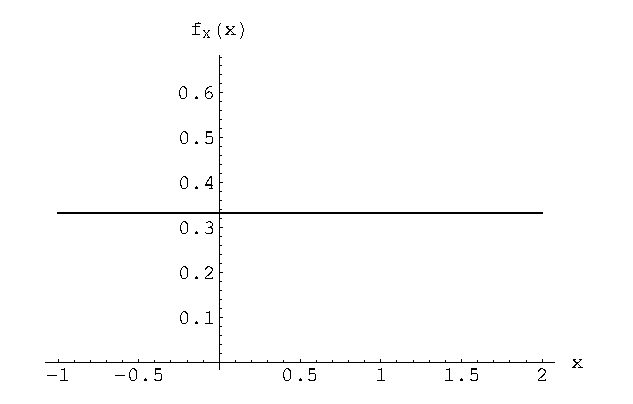
\includegraphics[scale=0.75]{densidaduniforme12}
&

       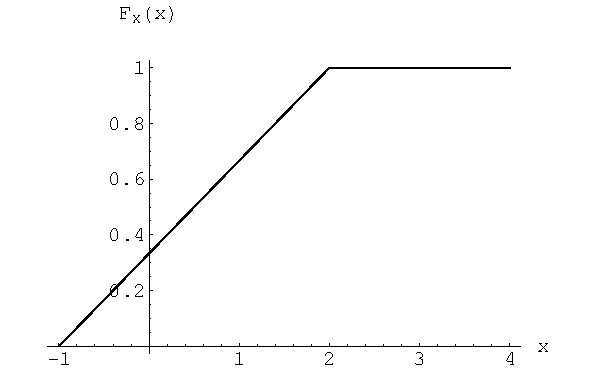
\includegraphics[scale=0.75]{distribucionuniforme12}\\ a) & b) \end{tabular}
\end{center}
       \caption{ Gráficas de la función de densidad (a)  y de la función de distribución (b) de una v.a. $U(-1,2)$.}
        \end{figure}%%%%%%%%  Sea $X$ una v.a. continua diremos que tiene distribución
%%%%%%%%          uniforme en el intervalo $(a,b)$ si su función de distribución
%%%%%%%%          es
%%%%%%%%          $$F_{X}(x)=\left\{\begin{array}{ll} 0 & \mbox{ si } x\leq a\\
%%%%%%%%          \frac{x-a}{b-a} & \mbox{ si } a\leq x\leq\\
%%%%%%%%          1 & \mbox{ si } b\leq x\end{array}\right.$$
%%%%%%%%
%%%%%%%%          $F$ es absolutamente continua y tiene por densidad:
%%%%%%%%         $$f_{X}(x)=\left\{\begin{array}{ll} \frac{1}{b-a} & \mbox{ si }
%%%%%%%%         a<x<b\\
%%%%%%%%         0 & \mbox{en el resto de casos}\end{array}\right.$$
\end{frame}

\begin{frame}



\subsubsection{Cambio lineal v.a. uniforme}


Si $X$ sigue una distribución $U(a,b)$ entonces  $Z=\frac{x-a}{b-a}$ sigue una distribución $U(0,1)$.

En general si $d$ y $e$ son dos constantes reales  $T=d\cdot X+e$ sigue una ley $U(d\cdot a +e,d\cdot b +e)$  si $d>0$, cuando $d$ sea negativo $T$ sigue una ley 
$U(d\cdot b +e,d\cdot a +e)$. Las demostración se dejan como ejercicios.

\end{frame}

\begin{frame}


\subsubsection{Resumen v.a con distribución uniforme, $U(a,b)$}

\scriptsize
\begin{tabular}{|c|c|c|c|c|}
\hline \begin{tabular}{c} Valores\\ admisibles.\end{tabular} & $f_{X}(x)$ & $F_X(x)=P(X\leq
X)=$ &
 $E(X)$ & $Var(X)$\\\hline & & & &\\
 $D_X=(a,b)$ & $\left\{\begin{array}{ll}
\frac{1}{b-a} & \mbox{si } a<x<b\\ 0  & \mbox{en cualquier otro caso}
\end{array}
\right.$  &  $\left\{\begin{array}{ll} 0 & \mbox{ si } x\leq a\\
          \frac{x-a}{b-a} & \mbox{ si } a\leq x\leq\\
          1 & \mbox{ si } b\leq x\end{array}\right.$
 & $\frac{a+b}{2}$ & $\frac{(b-a)^2}{12}$ \\& & & &\\ \hline
\end{tabular}

\normalsize

\end{frame}

\begin{frame}


         \subsection{Distribución exponencial (exponencial negativa):}
         Supongamos que tenemos un proceso Poisson con parámetro
         $\lambda$ en una unidad de tiempo.

         Sea $t$ una cantidad de tiempo en u.t. entonces $N_{t}=$ número de
         eventos en el intervalo de tiempo $(0,t]$
         es una $Po(\lambda\cdot t)$. Consideremos la v.a.
         $T=$tiempo transcurrido entre dos eventos Poisson consecutivos.

         Sea $t>0$, entonces
         $$P(T>t)=P(\mbox{Cero eventos en el
         intervalo}(0,t])
         =P(N_{t}=0)=
         \frac{(\lambda t)^0}{0!} e^{-\lambda
         t}=e^{-\lambda t}.$$

\end{frame}

\begin{frame}

         Tomando complementarios, la función de distribución de $T$ será

         $$F_{T}(t)=P(T\leq t)=\left\{\begin{array}{ll} 0 &\mbox{ si } t\leq 0\\
          1-P(T>t)=1-e^{-\lambda t}& \mbox{ si } t>0\end{array}\right.$$

         Entonces

         $$f_{T}(t)=\left\{\begin{array}{ll}
         \lambda e^{-\lambda t} & \mbox{ si }  t>0\\
         0 & \mbox{ si } t\leq 0
         \end{array}\right.$$

         La exponencial se denota por $Exp(\lambda)$
\end{frame}

\begin{frame}

\subsubsection{Propiedad de la falta de memoria}

          Sea $X$  una v.a. $Exp(\lambda)$ entonces

          $$P(X>s+t/X>s)=P(X>t)\mbox{  para todo } s,t\in \RR$$

          Toda v.a. absolutamente continua, que tome valores positivos
          y que verifique la propiedad de la falta de memoria es una v.a.
          exponencial.


\end{frame}

\begin{frame}

\subsubsection{Resumen v.a con distribución exponencial, $Exp(\lambda)$}

Sea $X\equiv Exp(\lambda).$

\scriptsize
\begin{tabular}{|c|c|c|c|c|}
\hline \begin{tabular}{c} Valores\\ admisibles.\end{tabular} & $f_{X}(x)$ & $F_X(x)=P(X\leq
X)=$ &
 $E(X)$ & $Var(X)$\\\hline & & & &\\
 $D_X=(0,+\infty)$ & $\left\{\begin{array}{ll}
         \lambda e^{-\lambda x} & \mbox{ si }  x>0\\
         0 & \mbox{ si } x\leq 0
         \end{array}\right.$ &  $F_{X}(x)=P(X\leq x)=\left\{\begin{array}{ll} 0 &\mbox{si } x\leq 0\\
          1-e^{-\lambda x}& \mbox{si } x>0\end{array}\right.
$ & $\frac{1}{\lambda}$ & $\frac{1}{\lambda^2}$ \\& & & &\\ \hline
\end{tabular}

\normalsize


\end{frame}

\begin{frame}


          \subsection{Distribución normal o Gaussiana}


          Diremos que una v.a. $X$ sigue una ley normal de parámetros
          $\mu$ y $\sigma^2$ y lo denotaremos por $N(\mu,\sigma^2)$
          si tiene por función de densidad

          $$f_{X}(x)=\frac{1}{\sqrt{2\pi}\sigma}
          e^{\frac{-(x-\mu)^2}{2\sigma^{2}}}\mbox{ para todo }x\in \RR$$

          La gráfica de esta función es la conocida campana de Gauss.

          La v.a. normal con $\mu=0$ y $\sigma=1$ recibe el nombre de
          normal estándar y se suele denotar por la letra $Z$.


%%%%%%%%          \textbf{Propiedad} Sea $X$ una v.a. $N(\mu,\sigma^2)$ y sea
%%%%%%%%          $f_{X}$ su función de densidad. Entonces:
%%%%%%%%          \vskip -1cm
%%%%%%%%          \begin{enumerate}[a)]
%%%%%%%%          \item Evidentemente $f_{X}$ verifica todas las pro\-pie\-da\-des de las
%%%%%%%%          funciones de densidad.
%%%%%%%%          \item $f_{X}(\mu-x)=f_{X}(\mu+x)$ es simétrica respecto de la recta
%%%%%%%%          $x=\mu$
%%%%%%%%          \item $f_{X}$ alcanza el máximo en $x=\mu$
%%%%%%%%         \item Si $F_{X}$ la función de distribución de $X$ entonces
%%%%%%%%         $F_{X}(\mu+x)=1-F_{X}(\mu-x)$. En par\-ti\-cu\-lar si $Z$ es una
%%%%%%%%         $N(0,1)$ entonces $F_{Z}(-x)=1-F_{Z}(x)$
%%%%%%%%         \item $Z=\frac{X-\mu}{\sigma}$ es una v.a. $N(0,1)$ y
%%%%%%%%              $X=\sigma Z+\mu$ es una $N(\mu,\sigma^{2})$ donde $Z$ es la
%%%%%%%%              normal estándar.
%%%%%%%%
%%%%%%%%          \end{enumerate}
%%%%%%%%



%%%%%%%%\section{La distribución normal o de Gauss}
%%%%%%%%
%%%%%%%% Diremos que una v.a. continua $X$ tiene
%%%%%%%%distribución normal con parámetros $\mu$ y  $\sigma^{2}$ a una variable aleatoria que tenga
%%%%%%%%por función de densidad :
%%%%%%%%$$f(x)={1\over{\sqrt{2\pi}\sigma}} {e\vphantom{A}}^{\left(-{1\over
%%%%%%%%2}{\left({x-\mu}\over{\sigma}\right)}^{2}\right)}$$
\end{frame}

\begin{frame}



\begin{figure}[h]
\begin{center}
\begin{tabular}{cc}
 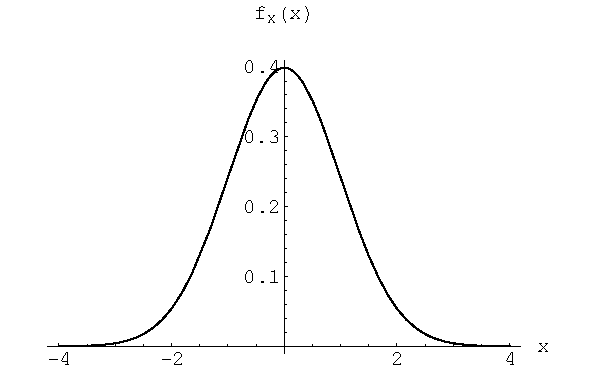
\includegraphics[scale=0.75]{densidadgaussiana}
&
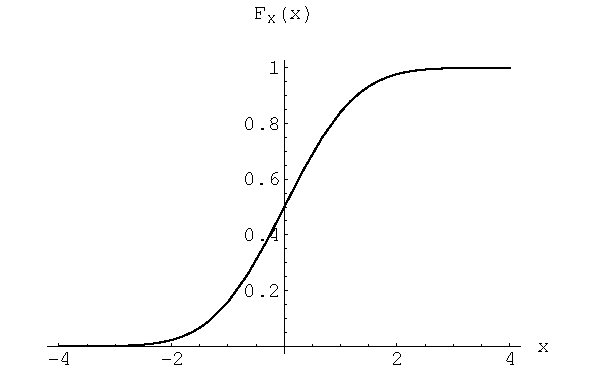
\includegraphics[scale=0.75]{distribuciongaussiana}\\ a) & b) \end{tabular}
\end{center}
       \caption{Gráficas de la función de densidad (a)  y de la  función de distribución (b) de una v.a. $N(0,1)$.}
        \end{figure}


%%%%%%%%\begin{figure}
%%%%%%%%\begin{center}
%%%%%%%%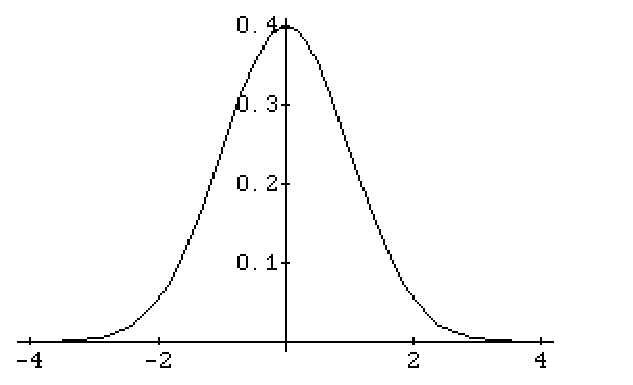
\includegraphics{normal.eps}
%%%%%%%%\end{center}
%%%%%%%%\caption{Curva de Gauss con $\mu=0$ y $\sigma=1$ }
%%%%%%%%\end{figure}

\end{frame}

\begin{frame}


Su función de distribución es, como sabemos :
$$F(x)=\int_{-\infty}^{x} {1\over{\sqrt{2\pi}\sigma}}
{e\vphantom{A}}^{-{1\over 2}{\left({t-\mu}\over{\sigma}\right)}^{2}} dt$$

Que no tiene ninguna expresión algebraica ``decente''. Es por esta razón, y  por comodidad,
que esta función está tabulada.



Cuando una variable tiene distribución normal con parámetros $\mu,\sigma$ la denotamos por
$X\equiv N(\mu,\sigma^2)$

\end{frame}

\begin{frame}

\subsubsection{Resumen v.a con distribución normal, $N(\mu,\sigma^2)$}

\scriptsize
\begin{tabular}{|c|c|c|c|c|}
\hline \begin{tabular}{c} Valores\\ admisibles.\end{tabular} & $f_{X}(x)$ & $F_X(x)=P(X\leq
X)=$ &
 $E(X)$ & $Var(X)$\\\hline & & & &\\
 $D_X=\RR$ & $=\frac{1}{\sqrt{2\pi}\sigma}
          e^{\frac{-(x-\mu)^2}{2\sigma^{2}}}\mbox{ para todo }x\in \RR$ & Tabulada la
          $N(0,1)$ & $\mu$ & $\sigma^2$ \\& & & &\\ \hline
\end{tabular}
\normalsize

\end{frame}

\begin{frame}


\subsubsection{Propiedades de la distribución normal.} La función de densidad de la
distribución normal tiene las siguientes propiedades:
\begin{enumerate}[a)]
\item $f$ es continua
\item $\int_{-\infty}^{+\infty} {1\over{\sqrt{2\pi}\sigma}} {e\vphantom{A}}^{-{1\over
2}{\left({x-\mu}\over{\sigma}\right)}^{2}} dx =1$ ( propiedad de todas las densidades).
\item $f(\mu+x)=f(\mu-x)$ y $F(x+\mu)=1-F(\mu-x)$ para todo $x\in \cal{R}$
\item $\lim\limits_{x\to+\infty}f(x)=\lim\limits_{x\to-\infty}f(x)=0$
es decir tiene asíntota horizontal a derecha e izquierda.
\item $f$ es estrictamente creciente si $x<\mu$ y decreciente si $x>\mu$.
\item Alcanza el máximo en $x=\mu$ y en este punto vale $f(\mu)=\frac{1}{\sqrt{2\pi}\sigma}$
\item Tiene dos puntos de inflexión en $x=\mu+\sigma$ y en $x=\mu-\sigma$.
\end{enumerate}
\end{frame}

\begin{frame}


\subsubsection{Transformaciones lineales de variables aleatorias normales}

\begin{prop} Sea $X\equiv N(\mu,\sigma^2)$  entonces la variable $Y=a X+b$ con
$a\not=0,b\in\cal{R}$ tiene distribución $N(a\mu+b, a^2 \sigma^2)$

En particular si  $X\equiv N(\mu,\sigma^2)$, tomando $a=\frac{1}{\sigma}$ y $b=
\frac{-\mu}{\sigma}$ la v.a. $Z={{X-\mu}\over {\sigma}}$ se distribuye $N(0,1)$.

Esta propiedad es muy importante, ya que utilizándola sólo necesitaremos tabular la
$N(0,1)$. A la función de distribución de una $Z\equiv N(0,1)$ la llamaremos $F_Z$  y a una
normal $N(0,1)$  se le denomina normal estándar. Por lo tanto si
$F_X(x)=F_Z(\frac{x-\mu}{\sigma})$.
\end{prop} 

La propiedad siguiente se desprende de las propiedades generales de una normal y nos será
muy útil en los cálculos de probabilidades de una normal.
\end{frame}

\begin{frame}

\textbf{Propiedad} Si $Z\equiv N((0,1)$ entonces $F_{Z}(x)=1-F_{Z}(-x)$.

\begin{example} Sea $Z\equiv N(0,1)$  Calcular :
\begin{enumerate}[a)]
\item Dado $\delta>0$, $P(-\delta\leq Z \leq
\delta)=F_{Z}(\delta)-F_{Z}(-\delta)=F_Z(3)-(1-F_Z(\delta))=2 F_Z(\delta)-1$
\item $P(-4\leq Z \leq 4)=F_{Z}(4)-F_{Z}(-4)=2 F_Z(4)-1$
\item $P(-2\leq Z \leq 2)=F_{Z}(2)-F_{Z}(-2)=2 F_Z(2)-1$
\item $P(Z\leq -2)=F_Z(-2)=1-F_Z(2)$
\item $P( Z \leq 2)=F_{Z}(2)$
\item $P( Z \geq 2)=1-P(Z<2)=1-F_{Z}(2)$
\item $P( Z > 2)=1-P(Z\leq 2)=1-F_{Z}(2)$
\item $P( Z = 2)=0$
\item $P( Z \geq -2)=1-P(Z< -2)=1-F_{Z}(-2)=1-(1-F_Z(2))=F_Z(2).$
\end{enumerate}
\end{example}


\end{frame}

\begin{frame}

    Resumiendo podemos utilizar las siguientes propiedades, $X\equiv N(\mu,\sigma)$
    \begin{itemize}
    \item  $Z$ es su variable tipificada, es decir,
    $Z=\frac{X-\mu}{\sigma}\equiv N(0,1)$ entonces:

    $$P(X\leq x)=P(\frac{X-\mu}{\sigma}\leq
    \frac{x-\mu}{\sigma})=F_{Z}(\frac{x-\mu}{\sigma})$$

   \item  Cuando tengamos un intervalo
    $$P(a<X<b)=P(\frac{a-\mu}{\sigma}<\frac{X-\mu}{\sigma}<\frac{b-\mu}{\sigma})=$$

    $$=P(\frac{a-\mu}{\sigma}<Z<\frac{b-\mu}{\sigma})=F_{Z}(\frac{b-\mu}{\sigma})-
    F_{Z}(\frac{a-\mu}{\sigma})$$
    \item Si $\delta>0$ $P(\mu-\delta\leq X \leq
\mu+\delta)=2 F_Z(\frac{\delta}{\sigma})-1$
\end{itemize}
\end{frame}
%\end{document}
\begin{frame}

\frametitle{Ejemplo}
Sea $X$ una normal com media $2$ y varianza $4$, entonces
\begin{enumerate}[a)]
\item  $P(1< X< 2)= P(\frac{1-2}{2}<\frac{X-2}{2}<\frac{2-2}{2})=P(\frac{-1}{2}<Z<0)=F_{Z}(0)-F_{Z}(-0.5)=\frac{1}{2}-1+F_{Z}(0.5).$
\item $P(X>3)=P(\frac{X-2}{2}>\frac{3-2}{2})=P(Z>0.5)=1-F_{Z}(0.5).$
\end{enumerate}
\end{frame}

\end{document}
